% Study interfaces only; backend alternatives and evaluation labels are explicit.
\documentclass[tikz,border=2pt]{standalone}
\usepackage{fontspec}
\setsansfont{Arial}
\usetikzlibrary{arrows.meta}
\definecolor{blue}{HTML}{0072B2}
\definecolor{orange}{HTML}{B36B00}
\definecolor{ink}{HTML}{303843}
\begin{document}
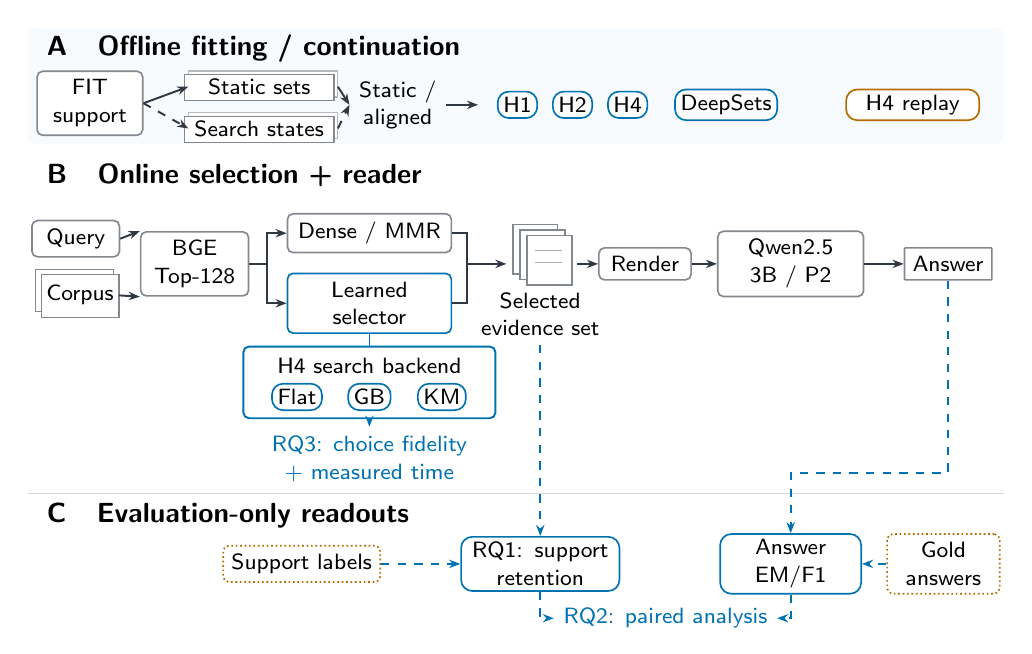
\begin{tikzpicture}[x=1cm,y=1cm,font=\sffamily\fontsize{8.5}{10}\selectfont,
 box/.style={draw=ink!60,fill=white,rounded corners=2pt,align=center,inner sep=3pt,line width=.6pt},
 badge/.style={box,rounded corners=4pt,draw=blue,inner sep=2pt},
 flow/.style={-{Stealth[length=4pt]},line width=.7pt,draw=ink},
 readout/.style={flow,draw=blue,dashed},
 head/.style={anchor=west,font=\sffamily\bfseries\fontsize{10}{11}\selectfont}]
\path[use as bounding box] (0,0) rectangle (12.4,7.6);
\fill[blue!3,rounded corners=3pt] (0,6.12) rectangle (12.4,7.6);
\node[head] at (.12,7.34) {A\quad Offline fitting / continuation};
\node[box,text width=1.13cm] (fit) at (.79,6.64) {FIT support};
% Small offset evidence cards distinguish the two training sources.
\foreach \y in {6.85,6.32} {
 \draw[ink!35,fill=white] (2.04,\y-.13) rectangle (3.94,\y+.20);
 \draw[ink!60,fill=white] (1.99,\y-.18) rectangle (3.89,\y+.15);
}
\node at (2.94,6.85) {Static sets};
\node at (2.94,6.32) {Search states};
\draw[flow] (fit.east)--(2.04,6.85);
\draw[flow,dashed] (fit.east)--(2.04,6.32);
\node[align=center] (train) at (4.7,6.62) {Static /\\aligned};
\draw[flow] (3.94,6.85)--(train.west);
\draw[flow,dashed] (3.94,6.32)--(train.west);
\draw[flow] (train.east)--(5.72,6.62);
\foreach \x/\label in {6.22/H1,6.92/H2,7.62/H4,8.87/DeepSets}
 \node[badge] at (\x,6.62) {\label};
\node[badge,draw=orange,text width=1.55cm] at (11.24,6.62) {H4 replay};

\node[head] at (.12,5.72) {B\quad Online selection + reader};
\node[box,text width=.9cm] (query) at (.61,4.92) {Query};
\draw[ink!60,fill=white] (.1,3.99) rectangle (1.09,4.53);
\draw[ink!60,fill=white] (.17,3.92) rectangle (1.16,4.46);
\node at (.665,4.2) {Corpus};
\node[box,text width=1.16cm] (bge) at (2.12,4.6) {BGE\\Top-128};
\draw[flow] (query.east)--(bge.north west);
\draw[flow] (1.16,4.2)--(bge.south west);
\node[box,text width=1.87cm] (base) at (4.34,4.99) {Dense / MMR};
\node[box,draw=blue,text width=1.87cm] (learn) at (4.34,4.10) {Learned selector};
\coordinate (split) at (3.04,4.6);
\draw[ink,line width=.7pt] (bge.east)--(split);
\draw[flow] (split)|-(base.west);
\draw[flow] (split)|-(learn.west);
\coordinate (merge) at (5.58,4.6);
\draw[ink,line width=.7pt] (base.east)-|(merge);
\draw[ink,line width=.7pt] (learn.east)-|(merge);
% Three offset paragraph cards, with line marks and an explicit set label.
\foreach \x/\y in {6.16/4.47,6.25/4.40,6.34/4.33} {
 \draw[ink!60,fill=white,line width=.6pt] (\x,\y) rectangle +(.57,.63);
 \draw[ink!40,line width=.45pt] (\x+.10,\y+.44)--+(.35,0);
 \draw[ink!40,line width=.45pt] (\x+.10,\y+.29)--+(.35,0);
}
\node[align=center] at (6.51,3.96) {Selected\\evidence set};
\draw[flow] (merge)--(6.08,4.6);
\node[box,text width=.96cm] (render) at (7.84,4.6) {Render};
\draw[flow] (6.98,4.6)--(render.west);
\node[box,text width=1.64cm] (reader) at (9.69,4.6) {Qwen2.5\\3B / P2};
\draw[flow] (render.east)--(reader.west);
\node[box,rounded corners=.3pt] (answer) at (11.69,4.6) {Answer};
\draw[flow] (reader.east)--(answer.west);

% Nested execution alternatives, attached only to the learned H4 selector.
\draw[blue,rounded corners=2pt,line width=.7pt] (2.74,2.64) rectangle (5.94,3.55);
\node at (4.34,3.30) {H4 search backend};
\foreach \x/\label in {3.42/Flat,4.34/GB,5.26/KM}
 \node[badge] at (\x,2.91) {\label};
\draw[blue,line width=.6pt] (learn.south)--(4.34,3.55);
\node[align=center,text=blue] (rq3) at (4.34,2.12) {RQ3: choice fidelity\\+ measured time};
\draw[readout] (4.34,2.64)--(rq3.north);

\draw[ink!20] (0,1.68)--(12.4,1.68);
\node[head] at (.12,1.40) {C\quad Evaluation-only readouts};
\node[box,draw=orange,densely dotted] (labels) at (3.48,.79) {Support labels};
\node[badge,text width=1.87cm] (support) at (6.51,.79) {RQ1: support\\retention};
\node[badge,text width=1.65cm] (aeval) at (9.69,.79) {Answer EM/F1};
\node[box,draw=orange,densely dotted,text width=1.22cm] (gold) at (11.63,.79) {Gold\\answers};
\draw[readout] (6.51,3.57)--(support.north);
\draw[readout] (answer.south)--(11.69,1.95)--(9.69,1.95)--(aeval.north);
\draw[readout] (labels.east)--(support.west);
\draw[readout] (gold.west)--(aeval.east);
\node[align=center,text=blue] (rq2) at (8.1,.10) {RQ2: paired analysis};
\draw[readout] (support.south)|-(rq2.west);
\draw[readout] (aeval.south)|-(rq2.east);
\end{tikzpicture}
\end{document}
